\documentclass[11pt]{article}
%\usepackage{psfig}
\usepackage{latexsym}
\usepackage{amsfonts}
\usepackage{hyperref}
\usepackage{url}
\usepackage{listings}
% to use hyperlinks in References section
\hypersetup{urlbordercolor={1 1 1}}
\usepackage{graphicx}
\usepackage{listings}	

%define colors
\usepackage{xcolor} 	
\definecolor{dkgreen}{rgb}{0,0.6,0}
\definecolor{gray}{rgb}{0.5,0.5,0.5}
\definecolor{mauve}{rgb}{0.58,0,0.82}
\usepackage{graphicx}
\usepackage{hyperref}
\hypersetup{urlbordercolor={1 1 1}}
\DeclareGraphicsExtensions{.pdf,.jpg,.png,.eps}
\setlength{\textheight}{8.5in}
\setlength{\textwidth}{6.0in}
\setlength{\headheight}{0in}
\addtolength{\topmargin}{-.5in}
\addtolength{\oddsidemargin}{-.5in}

\usepackage{url}
\def\UrlBreaks{\do\A\do\B\do\C\do\D\do\E\do\F\do\G\do\H\do\I\do\J
\do\K\do\L\do\M\do\N\do\O\do\P\do\Q\do\R\do\S\do\T\do\U\do\V
\do\W\do\X\do\Y\do\Z\do\[\do\\\do\]\do\^\do\_\do\`\do\a\do\b
\do\c\do\d\do\e\do\f\do\g\do\h\do\i\do\j\do\k\do\l\do\m\do\n
\do\o\do\p\do\q\do\r\do\s\do\t\do\u\do\v\do\w\do\x\do\y\do\z
\do\.\do\@\do\\\do\/\do\!\do\_\do\|\do\;\do\>\do\]\do\)\do\,
\do\?\do\'\do+\do\=\do\#} 

\newenvironment{cvl}{\begin{list}{$\bullet$}{
\setlength{\leftmargin}{0.3in} \setlength{\labelsep}{0.07in}
\setlength{\labelwidth}{0.17in} \setlength{\rightmargin}{0.0in}
\setlength{\topsep}{0.000in} \setlength{\partopsep}{0.000in}
\setlength{\parskip}{0.000in} \setlength{\parsep}{0.005in}
\setlength{\itemsep}{0.005in}}}{\end{list}}

\DeclareGraphicsExtensions{.pdf,.jpg,.png,.eps}
\usepackage[T1]{fontenc}	%special characters copy-able
\usepackage{xspace}
% \usepackage{times}
\usepackage{enumerate}
\newcommand{\espoofer}{{\sf espoofer}\space}
\newcommand{\dmark}{{\sf DMARC}\space}
\newcommand{\dkim}{{\sf DKIM}\space}
\newcommand{\spf}{{\sf SPF}\space}
\newcommand{\tor}{{\sf Tor}\xspace}
\newcommand{\torbw}{{\sf Tor Browser}\xspace}
\newcommand{\darkweb}{{\sf DarkWeb}\xspace}
\definecolor{myblue}{HTML}{1F5AB4}%1F5AB4
\hypersetup{colorlinks,urlcolor=black,linkcolor=myblue,anchorcolor=black,citecolor=red}
%--------------
%% Modified by Zhiqiang Lin
%% 01/18/2012
%%
%% Template file was from http://www.cs.umd.edu/~jkatz
%%
%% preamble.tex
%% this should be included with a command like
%% %--------------
%% Modified by Zhiqiang Lin
%% 01/18/2012
%%
%% Template file was from http://www.cs.umd.edu/~jkatz
%%
%% preamble.tex
%% this should be included with a command like
%% %--------------
%% Modified by Zhiqiang Lin
%% 01/18/2012
%%
%% Template file was from http://www.cs.umd.edu/~jkatz
%%
%% preamble.tex
%% this should be included with a command like
%% \input{preamble.tex}
%% \lecture{``lecture number''}{``date''}{``name of professor''}{``name
%%  of student''}

\hbadness=10000
\vbadness=10000

\newcommand{\handout}[5]{
   \renewcommand{\thepage}{#1-\arabic{page}}
   \noindent
   \begin{center}
   \framebox{
      \vbox{
    \hbox to 5.78in { {\bf CSE 5473 --- Network Security} 
     	 \hfill #2 }
       \vspace{4mm}
       \hbox to 5.78in { {\Large \hfill #5  \hfill} }
       \vspace{2mm}
       \hbox to 5.78in { {\it #3 \hfill #4} }
      }
   }
   \end{center}
   \vspace*{4mm}
}

\newcommand{\lecture}[4]{\handout{#1}{#2}{#3}{#4}{#1}}
%\newcommand{\lecture}[4]{\handout{#1}{#2}{Lecturer: #3}{Scribe(s): #4}{Lecture #1}}

\def\epsilon{\varepsilon}
\def\phi{\varphi}
\def\bool{\{0,1\}}
\def\poly{{\sf poly}}
\def\cross{\times}

\newcommand{\xor}{\oplus}
\newcommand{\Xor}{\bigoplus}
\newcommand{\ceil}[1]{\left\lceil {#1} \right\rceil}
\newcommand{\floor}[1]{\left\lfloor #1 \right\rfloor}
\newcommand{\ignore}[1]{}
\newcommand{\integers}[1]{{\mathbb Z}_{#1}}
\newcommand{\bydef}{\stackrel{\rm def}{=}}
\newcommand{\isequal}{\stackrel{\rm ?}{=}}
\newcommand{\compeq}{\stackrel{\rm c}{\equiv}} % computationally indistinguishable

\newcommand{\qed}{\hspace*{\fill}\rule{7pt}{7pt}}
\newenvironment{proof_sketch}{\noindent{\bf Sketch of Proof} (Informal)\hspace*{1em}}{\qed\medskip}
\newenvironment{proof}{\noindent{\bf Proof}\hspace*{1em}}{\qed\medskip}
\newenvironment{proofof}[1]{\noindent{\bf Proof} of #1:\hspace*{1em}}{\qed\medskip}
%\newenvironment{claim}{\noindent{\bf Claim}\hspace*{1em}\begin{em}}{\end{em}\medskip}
\newcounter{defcounter}
\setcounter{defcounter}{1}
\newenvironment{definition}{\medskip\noindent{\bf Definition \thedefcounter}}{\hspace*{\fill}$\diamondsuit$\stepcounter{defcounter}\medskip}
\newtheorem{theorem}{Theorem}
\newtheorem{corollary}[theorem]{Corollary}
\newtheorem{lemma}[theorem]{Lemma}
\newtheorem{claim}[theorem]{Claim}
\newtheorem{fact}[theorem]{Fact}
\newtheorem{conjecture}[theorem]{Conjecture}
\newenvironment{assumption}{\noindent{\bf Assumption}\hspace*{1em}\begin{em}}{\end{em}\medskip}
\newenvironment{remark}{\noindent{\bf Remark}\hspace*{1em}}{\bigskip}

\ignore{
\newcommand{\FOR}{{\bf for}}
\newcommand{\TO}{{\bf to}}
\newcommand{\DO}{{\bf do}}
\newcommand{\WHILE}{{\bf while}}
\newcommand{\AND}{{\bf and}}
\newcommand{\IF}{{\bf if}}
\newcommand{\THEN}{{\bf then}}
\newcommand{\ELSE}{{\bf else}}

%%% You probably will not need to use the commands listed below

\makeatletter
\def\fnum@figure{{\bf Figure \thefigure}}
\def\fnum@table{{\bf Table \thetable}}
\long\def\@mycaption#1[#2]#3{\addcontentsline{\csname
  ext@#1\endcsname}{#1}{\protect\numberline{\csname 
  the#1\endcsname}{\ignorespaces #2}}\par
  \begingroup
    \@parboxrestore
    \small
    \@makecaption{\csname fnum@#1\endcsname}{\ignorespaces #3}\par
  \endgroup}
\def\mycaption{\refstepcounter\@captype \@dblarg{\@mycaption\@captype}}
\makeatother

\newcommand{\figcaption}[1]{\mycaption[]{#1}}
\newcommand{\tabcaption}[1]{\mycaption[]{#1}}
\newcommand{\head}[1]{\chapter[Lecture \##1]{}}
\newcommand{\mathify}[1]{\ifmmode{#1}\else\mbox{$#1$}\fi}
\def\half{\frac{1}{2}}

\newcommand{\fig}[4]{
        \begin{figure}
        \setlength{\epsfysize}{#2}
        \vspace{3mm}
        \centerline{\epsfbox{#4}}
        \caption{#3} \label{#1}
        \end{figure}
        }
}



%% \lecture{``lecture number''}{``date''}{``name of professor''}{``name
%%  of student''}

\hbadness=10000
\vbadness=10000

\newcommand{\handout}[5]{
   \renewcommand{\thepage}{#1-\arabic{page}}
   \noindent
   \begin{center}
   \framebox{
      \vbox{
    \hbox to 5.78in { {\bf CSE 5473 --- Network Security} 
     	 \hfill #2 }
       \vspace{4mm}
       \hbox to 5.78in { {\Large \hfill #5  \hfill} }
       \vspace{2mm}
       \hbox to 5.78in { {\it #3 \hfill #4} }
      }
   }
   \end{center}
   \vspace*{4mm}
}

\newcommand{\lecture}[4]{\handout{#1}{#2}{#3}{#4}{#1}}
%\newcommand{\lecture}[4]{\handout{#1}{#2}{Lecturer: #3}{Scribe(s): #4}{Lecture #1}}

\def\epsilon{\varepsilon}
\def\phi{\varphi}
\def\bool{\{0,1\}}
\def\poly{{\sf poly}}
\def\cross{\times}

\newcommand{\xor}{\oplus}
\newcommand{\Xor}{\bigoplus}
\newcommand{\ceil}[1]{\left\lceil {#1} \right\rceil}
\newcommand{\floor}[1]{\left\lfloor #1 \right\rfloor}
\newcommand{\ignore}[1]{}
\newcommand{\integers}[1]{{\mathbb Z}_{#1}}
\newcommand{\bydef}{\stackrel{\rm def}{=}}
\newcommand{\isequal}{\stackrel{\rm ?}{=}}
\newcommand{\compeq}{\stackrel{\rm c}{\equiv}} % computationally indistinguishable

\newcommand{\qed}{\hspace*{\fill}\rule{7pt}{7pt}}
\newenvironment{proof_sketch}{\noindent{\bf Sketch of Proof} (Informal)\hspace*{1em}}{\qed\medskip}
\newenvironment{proof}{\noindent{\bf Proof}\hspace*{1em}}{\qed\medskip}
\newenvironment{proofof}[1]{\noindent{\bf Proof} of #1:\hspace*{1em}}{\qed\medskip}
%\newenvironment{claim}{\noindent{\bf Claim}\hspace*{1em}\begin{em}}{\end{em}\medskip}
\newcounter{defcounter}
\setcounter{defcounter}{1}
\newenvironment{definition}{\medskip\noindent{\bf Definition \thedefcounter}}{\hspace*{\fill}$\diamondsuit$\stepcounter{defcounter}\medskip}
\newtheorem{theorem}{Theorem}
\newtheorem{corollary}[theorem]{Corollary}
\newtheorem{lemma}[theorem]{Lemma}
\newtheorem{claim}[theorem]{Claim}
\newtheorem{fact}[theorem]{Fact}
\newtheorem{conjecture}[theorem]{Conjecture}
\newenvironment{assumption}{\noindent{\bf Assumption}\hspace*{1em}\begin{em}}{\end{em}\medskip}
\newenvironment{remark}{\noindent{\bf Remark}\hspace*{1em}}{\bigskip}

\ignore{
\newcommand{\FOR}{{\bf for}}
\newcommand{\TO}{{\bf to}}
\newcommand{\DO}{{\bf do}}
\newcommand{\WHILE}{{\bf while}}
\newcommand{\AND}{{\bf and}}
\newcommand{\IF}{{\bf if}}
\newcommand{\THEN}{{\bf then}}
\newcommand{\ELSE}{{\bf else}}

%%% You probably will not need to use the commands listed below

\makeatletter
\def\fnum@figure{{\bf Figure \thefigure}}
\def\fnum@table{{\bf Table \thetable}}
\long\def\@mycaption#1[#2]#3{\addcontentsline{\csname
  ext@#1\endcsname}{#1}{\protect\numberline{\csname 
  the#1\endcsname}{\ignorespaces #2}}\par
  \begingroup
    \@parboxrestore
    \small
    \@makecaption{\csname fnum@#1\endcsname}{\ignorespaces #3}\par
  \endgroup}
\def\mycaption{\refstepcounter\@captype \@dblarg{\@mycaption\@captype}}
\makeatother

\newcommand{\figcaption}[1]{\mycaption[]{#1}}
\newcommand{\tabcaption}[1]{\mycaption[]{#1}}
\newcommand{\head}[1]{\chapter[Lecture \##1]{}}
\newcommand{\mathify}[1]{\ifmmode{#1}\else\mbox{$#1$}\fi}
\def\half{\frac{1}{2}}

\newcommand{\fig}[4]{
        \begin{figure}
        \setlength{\epsfysize}{#2}
        \vspace{3mm}
        \centerline{\epsfbox{#4}}
        \caption{#3} \label{#1}
        \end{figure}
        }
}



%% \lecture{``lecture number''}{``date''}{``name of professor''}{``name
%%  of student''}

\hbadness=10000
\vbadness=10000

\newcommand{\handout}[5]{
   \renewcommand{\thepage}{#1-\arabic{page}}
   \noindent
   \begin{center}
   \framebox{
      \vbox{
    \hbox to 5.78in { {\bf CSE 5473 --- Network Security} 
     	 \hfill #2 }
       \vspace{4mm}
       \hbox to 5.78in { {\Large \hfill #5  \hfill} }
       \vspace{2mm}
       \hbox to 5.78in { {\it #3 \hfill #4} }
      }
   }
   \end{center}
   \vspace*{4mm}
}

\newcommand{\lecture}[4]{\handout{#1}{#2}{#3}{#4}{#1}}
%\newcommand{\lecture}[4]{\handout{#1}{#2}{Lecturer: #3}{Scribe(s): #4}{Lecture #1}}

\def\epsilon{\varepsilon}
\def\phi{\varphi}
\def\bool{\{0,1\}}
\def\poly{{\sf poly}}
\def\cross{\times}

\newcommand{\xor}{\oplus}
\newcommand{\Xor}{\bigoplus}
\newcommand{\ceil}[1]{\left\lceil {#1} \right\rceil}
\newcommand{\floor}[1]{\left\lfloor #1 \right\rfloor}
\newcommand{\ignore}[1]{}
\newcommand{\integers}[1]{{\mathbb Z}_{#1}}
\newcommand{\bydef}{\stackrel{\rm def}{=}}
\newcommand{\isequal}{\stackrel{\rm ?}{=}}
\newcommand{\compeq}{\stackrel{\rm c}{\equiv}} % computationally indistinguishable

\newcommand{\qed}{\hspace*{\fill}\rule{7pt}{7pt}}
\newenvironment{proof_sketch}{\noindent{\bf Sketch of Proof} (Informal)\hspace*{1em}}{\qed\medskip}
\newenvironment{proof}{\noindent{\bf Proof}\hspace*{1em}}{\qed\medskip}
\newenvironment{proofof}[1]{\noindent{\bf Proof} of #1:\hspace*{1em}}{\qed\medskip}
%\newenvironment{claim}{\noindent{\bf Claim}\hspace*{1em}\begin{em}}{\end{em}\medskip}
\newcounter{defcounter}
\setcounter{defcounter}{1}
\newenvironment{definition}{\medskip\noindent{\bf Definition \thedefcounter}}{\hspace*{\fill}$\diamondsuit$\stepcounter{defcounter}\medskip}
\newtheorem{theorem}{Theorem}
\newtheorem{corollary}[theorem]{Corollary}
\newtheorem{lemma}[theorem]{Lemma}
\newtheorem{claim}[theorem]{Claim}
\newtheorem{fact}[theorem]{Fact}
\newtheorem{conjecture}[theorem]{Conjecture}
\newenvironment{assumption}{\noindent{\bf Assumption}\hspace*{1em}\begin{em}}{\end{em}\medskip}
\newenvironment{remark}{\noindent{\bf Remark}\hspace*{1em}}{\bigskip}

\ignore{
\newcommand{\FOR}{{\bf for}}
\newcommand{\TO}{{\bf to}}
\newcommand{\DO}{{\bf do}}
\newcommand{\WHILE}{{\bf while}}
\newcommand{\AND}{{\bf and}}
\newcommand{\IF}{{\bf if}}
\newcommand{\THEN}{{\bf then}}
\newcommand{\ELSE}{{\bf else}}

%%% You probably will not need to use the commands listed below

\makeatletter
\def\fnum@figure{{\bf Figure \thefigure}}
\def\fnum@table{{\bf Table \thetable}}
\long\def\@mycaption#1[#2]#3{\addcontentsline{\csname
  ext@#1\endcsname}{#1}{\protect\numberline{\csname 
  the#1\endcsname}{\ignorespaces #2}}\par
  \begingroup
    \@parboxrestore
    \small
    \@makecaption{\csname fnum@#1\endcsname}{\ignorespaces #3}\par
  \endgroup}
\def\mycaption{\refstepcounter\@captype \@dblarg{\@mycaption\@captype}}
\makeatother

\newcommand{\figcaption}[1]{\mycaption[]{#1}}
\newcommand{\tabcaption}[1]{\mycaption[]{#1}}
\newcommand{\head}[1]{\chapter[Lecture \##1]{}}
\newcommand{\mathify}[1]{\ifmmode{#1}\else\mbox{$#1$}\fi}
\def\half{\frac{1}{2}}

\newcommand{\fig}[4]{
        \begin{figure}
        \setlength{\epsfysize}{#2}
        \vspace{3mm}
        \centerline{\epsfbox{#4}}
        \caption{#3} \label{#1}
        \end{figure}
        }
}




\begin{document}


\lecture{Lab \#3}{Autumn 2020}{Understanding the Privacy with TOR and Bluetooth}{Due Nov 20th, 11:59PM}

\lstset{ %
   language=C,                % the language of the code
   basicstyle=\footnotesize\ttfamily,           % the size of the fonts that are used for the code
   literate={-}{-}1,
   columns=fullflexible,   %copy-paste-able
   %numbers=left,                   % where to put the line-numbers
   numberstyle=\tiny\color{gray},  % the style that is used for the line-numbers
   stepnumber=2,                   % the step between two line-numbers. If it's 1, each line 
                                   % will be numbered
   numbersep=5pt,                  % how far the line-numbers are from the code
   backgroundcolor=\color{white},      % choose the background color. You must add \usepackage{color}
   showspaces=false,               % show spaces adding particular underscores
   showstringspaces=false,         % underline spaces within strings
   showtabs=false,                 % show tabs within strings adding particular underscores
   frame=single,                   % adds a frame around the code
   rulecolor=\color{black},        % if not set, the frame-color may be changed on line-breaks within not-black text (e.g. commens (green here))
   tabsize=2,                      % sets default tabsize to 2 spaces
   captionpos=b,                   % sets the caption-position to bottom
   breaklines=true,                % sets automatic line breaking
   breakatwhitespace=false,        % sets if automatic breaks should only happen at whitespace
   title=\lstname,                   % show the filename of files included with \lstinputlisting;
                                   % also try caption instead of title
   keywordstyle=\color{blue},          % keyword style
   commentstyle=\color{dkgreen},       % comment style
   stringstyle=\color{mauve},         % string literal style
   escapeinside={\%*}{*)},            % if you want to add LaTeX within your code
   morekeywords={*,...}               % if you want to add more keywords to the set
 }
%%%% body goes in here %%%%

\section{Key Objectives}

 
\begin{itemize}
\item Reinforce your concept about data security and privacy. 
\item Get familiar with \tor and \tor based applications (i.e. \darkweb). 
\item Learn how to use \tor to protect your privacy.
\item Refresh your memory about Bluetooth workflow and privacy . 
\item Learn how to use tools to analyze Bluetooth traffic.

\end{itemize}

%In this project, you are required to use \tor and access \darkweb.   What you need to deliver is a report for this project. Details will be given in Section~\ref{deliver}. It is encouraged to finish the project individually.


%The project covers three common web application vulnerabilities: SQL injection, Cross-Site Scripting (XSS), and Shell Command Injection. According to the Open Web Application Security Project (OWASP) these vulnerabilities are in the top ten.


\section{Task~1: Experiment Setup}
 


\subsection{Install the Testing Platform}
 

\begin{enumerate}
\item Please install VMware:
\begin{itemize}
    \item If you are MacOS users, please download and install VMware Fusion. You can  download a free trial version (at \url{http://www.vmware.com/go/try-fusion-en}). For more details, please refer to \url{https://kb.vmware.com/s/article/2014097}. 
    \item If you are either Windows or Linux users, please download and install VMWare Station at \url{https://my.vmware.com/en/web/vmware/downloads/details?downloadGroup=PLAYER-1600&productId=1039&rPId=51984}.  

\end{itemize}
\item Please download the System Image at \url{https://drive.google.com/file/d/1MrouCQ5BxxQsj4Z0sH7TVryol6x3VHHi/view?usp=sharing}.

Please note that the System Image provided in this lab is different from the one used in lab\#2. This lab has all the required software installed and all the software can be found in ``/home/cse5473''. Therefore, if you download and import this System image into your VMware, you can \textbf{SKIP} the following software installation steps:
\begin{itemize}
\item \textbf{Installing \torbw}: You can use the following command to install \torbw: 
\begin{itemize}
\item Download \torbw at \url{https://www.torproject.org/dist/torbrowser/10.0.2/tor-browser-linux64-10.0.2_en-US.tar.xz}.
\item Unzip ``\texttt{tor-browser-linux64-10.0.2\_en-US.tar.xz}''.
 
\end{itemize}

\item \textbf{Install \textsf{whois}.} Whois is a tool for searching the specific information (e.g., current registrar, registrant information) of a specific domain. You can use the following command to install \textsf{whois}. 

\begin{lstlisting}
$ apt install whois
\end{lstlisting}\vspace{-6mm}
 
 \item \textbf{Install \tor service.} \tor service can anonymize all the traffic from your machine. You can use the following command to install \tor service. 
 \begin{lstlisting}
$ sudo apt install tor
\end{lstlisting}\vspace{-6mm}

\item \textbf{Install \textsf{Crackle}}: \textsf{Crackle} is a Bluetooth hacking tool which works against Bluetooth legacy (i.e., Bluetooth 4.0 and Bluetooth 4.1). It allows an attacker to brute force the TK (Temporary Key) and decrypt the encrypted Bluetooth packets.
\begin{itemize}
\item Download \textsf{Crackle} at \url{http://lacklustre.net/projects/crackle/crackle-0.1.tgz}.
\item Unzip \textsf{Crackle}.
 \begin{lstlisting}
tar -zxvf crackle-0.1.tgz
\end{lstlisting}\vspace{-6mm}
\item Install dependency using the following commands.
 \begin{lstlisting}
$ sudo apt-get install libpcap0.8-dev
\end{lstlisting}\vspace{-6mm}
\item Go to the directory of \textsf{Crackle} and type: 
 \begin{lstlisting}
$ make 
$ make install
\end{lstlisting}\vspace{-6mm}
\end{itemize}




\end{itemize}


 
 
\item Unzip and import the downloaded System Image into VMware (Check the link to see how to import the system image:  \url{https://docs.vmware.com/en/VMware-Workstation-Player-for-Linux/14.0/com.vmware.player.linux.using.doc/GUID-DDCBE9C0-0EC9-4D09-8042-18436DA62F7A.html}).

\item Login onto the system using the following credentials\footnote{Root user's password is 123456 as well}: 
 \begin{lstlisting}
Username: cse5473
Password: 123456
\end{lstlisting}\vspace{-6mm}


\section{Task~2: Understanding Identity Privacy via \tor and \torbw (50 Points)} 

\subsection{Using \torbw to visit \darkweb (20 Points)} 
\label{subsec:usetorbw}
\begin{enumerate}

\item Run \url{start-tor-browser.desktop}.
 \begin{lstlisting}
$ tar -zxvf tor-browser-linux64-10.0.2\_en-US.tar.xz
$ cd tor-browser_en-US
$ ./start-tor-browser.desktop
\end{lstlisting}\vspace{-6mm}
Ubuntu does not allow Root user to run \torbw, and you may want to log out Root user using the following command: 
 \begin{lstlisting}
$ exit
\end{lstlisting}\vspace{-6mm} 

\item Find available drakwebs at \url{https://www.thedarkweblinks.com/darknet-market-list/}. Copy one of the addresses to the address bar of \torbw and press ``ENTER'' (See \autoref{fig:dkwb}). 
% is a screenshot. 

\begin{figure}[h]
\centering
\frame{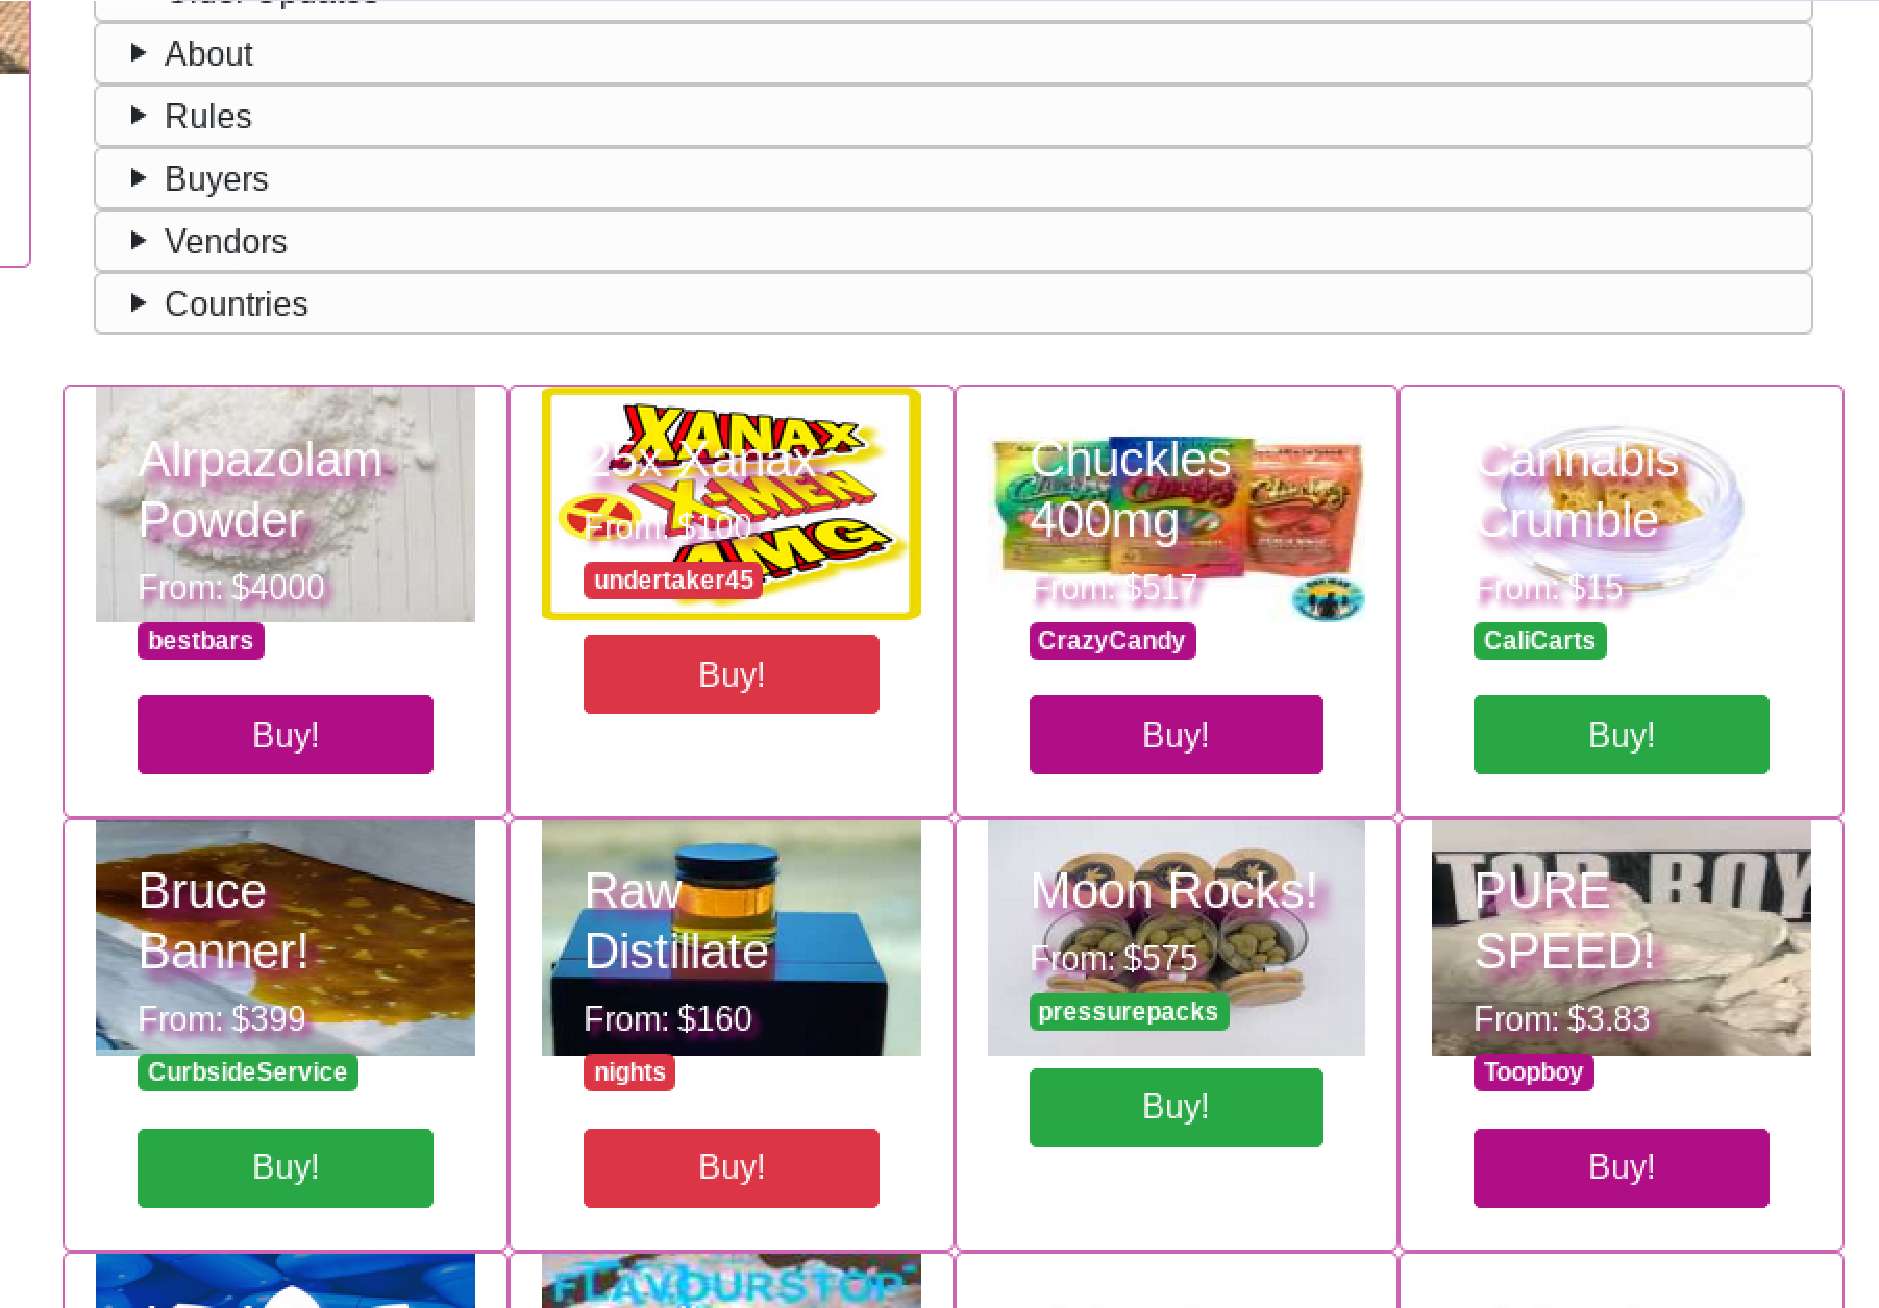
\includegraphics[width=0.8\columnwidth]{dkwb.pdf}}
\caption{Dark Market}\label{fig:dkwb}
\end{figure}


\textbf{Caution:} While browsing the dark webs, you should follow the following regulations:   
\begin{itemize}
\item Some dark webs may require registration before accessing the contents. Please do not provide any personal information. 
\item Always use your alias to communicate with other people in dark webs. 
\item Please do not buy anything from dark webs.
\item Please do not visit illegal content (e.g., child porn) on the dark webs.
\end{itemize}

\textbf{Question 1.} Put a screenshot into your report to show you have visited one of the dark webs successfully (5 points). 
 

\item Open your \textsf{Firefox} and visit \url{https://whatismyipaddress.com/} to check your IP address. Please remember the IP address, and we will use it later.   

 
\item Open your \torbw and visit \url{https://whatismyipaddress.com/} to check your IP address again.  

\textbf{Question 2.} Are the IP addresses displayed in step 3 and step 4 the same? If not, explain why (5 points). 

\item  Close your \textsf{Firefox}  and relaunch it again. Go to \url{https://whatismyipaddress.com/} to check your IP address.  

\item Close your \torbw and relaunch it again. Go to \url{https://whatismyipaddress.com/} to check your IP address again. 

\textbf{Question 3.} Are the IP addresses displayed in step 3 and step 5 the same? Are the IP addresses displayed in step 4 and step 6 the same? Please explain why (10 Points). 

 
\end{enumerate}

\subsection{Understanding \tor via ``whois'' command (10 points)} 
\begin{enumerate}

\item Check the information of \texttt{osu.edu} using \textsf{whois}:
 \begin{lstlisting}
$ whois osu.edu
\end{lstlisting}\vspace{-6mm}

\textbf{Question 1.} Put a screenshot into your report to show you have checked the information about \texttt{osu.edu} (5 points). 
 
\item Check the IP address of IP addresses displayed in \torbw (i.e., the IP addresses displayed in Section \ref{subsec:usetorbw}, Step 4 and Step 6) using \textsf{whois}.

\textbf{Question 2.} Put a screenshot into your report to show you have checked the IP addresses displayed in \torbw. Explain what you observed (5 points). 

Please note that the IP addresses displayed can be either an IPV4 address or an IPV6 address, and \textsf{whois} can handle both.  

\end{enumerate}

\subsection{Understanding \tor via \tor services (30 points)} 
\begin{enumerate}

\item You can start \tor services using the following commands: 
 \begin{lstlisting}
$ sudo service tor start
\end{lstlisting}\vspace{-6mm}


\item Check the status of your \tor services:
 \begin{lstlisting}
$ sudo service tor status
\end{lstlisting}\vspace{-6mm}

\textbf{Question 1.} Put a screenshot into your report to show \tor service has been launched successfully (10 points). 


\item You can also check the running status of \tor service by visiting the following URL in \textsf{Firefox}: \url{http://127.0.0.1:9050}.

\begin{figure}[h]
\centering
\frame{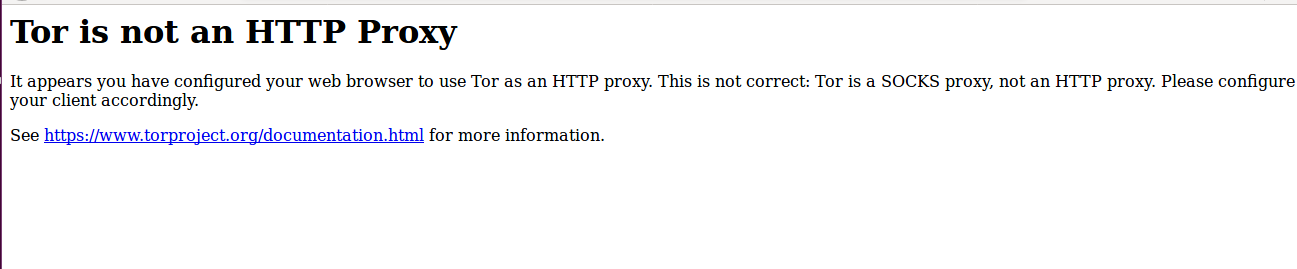
\includegraphics[width=0.8\columnwidth]{proxy.png}}
\caption{Check running status of the \tor service by using {\sf Firefox}}\label{fig:proxy}
\end{figure}

\item Configure your \textsf{Firefox} as follows. By doing that, we will use \tor services to tunnel the traffic (See \autoref{fig:proxyenable}). 

\begin{figure}[h]
\centering
\frame{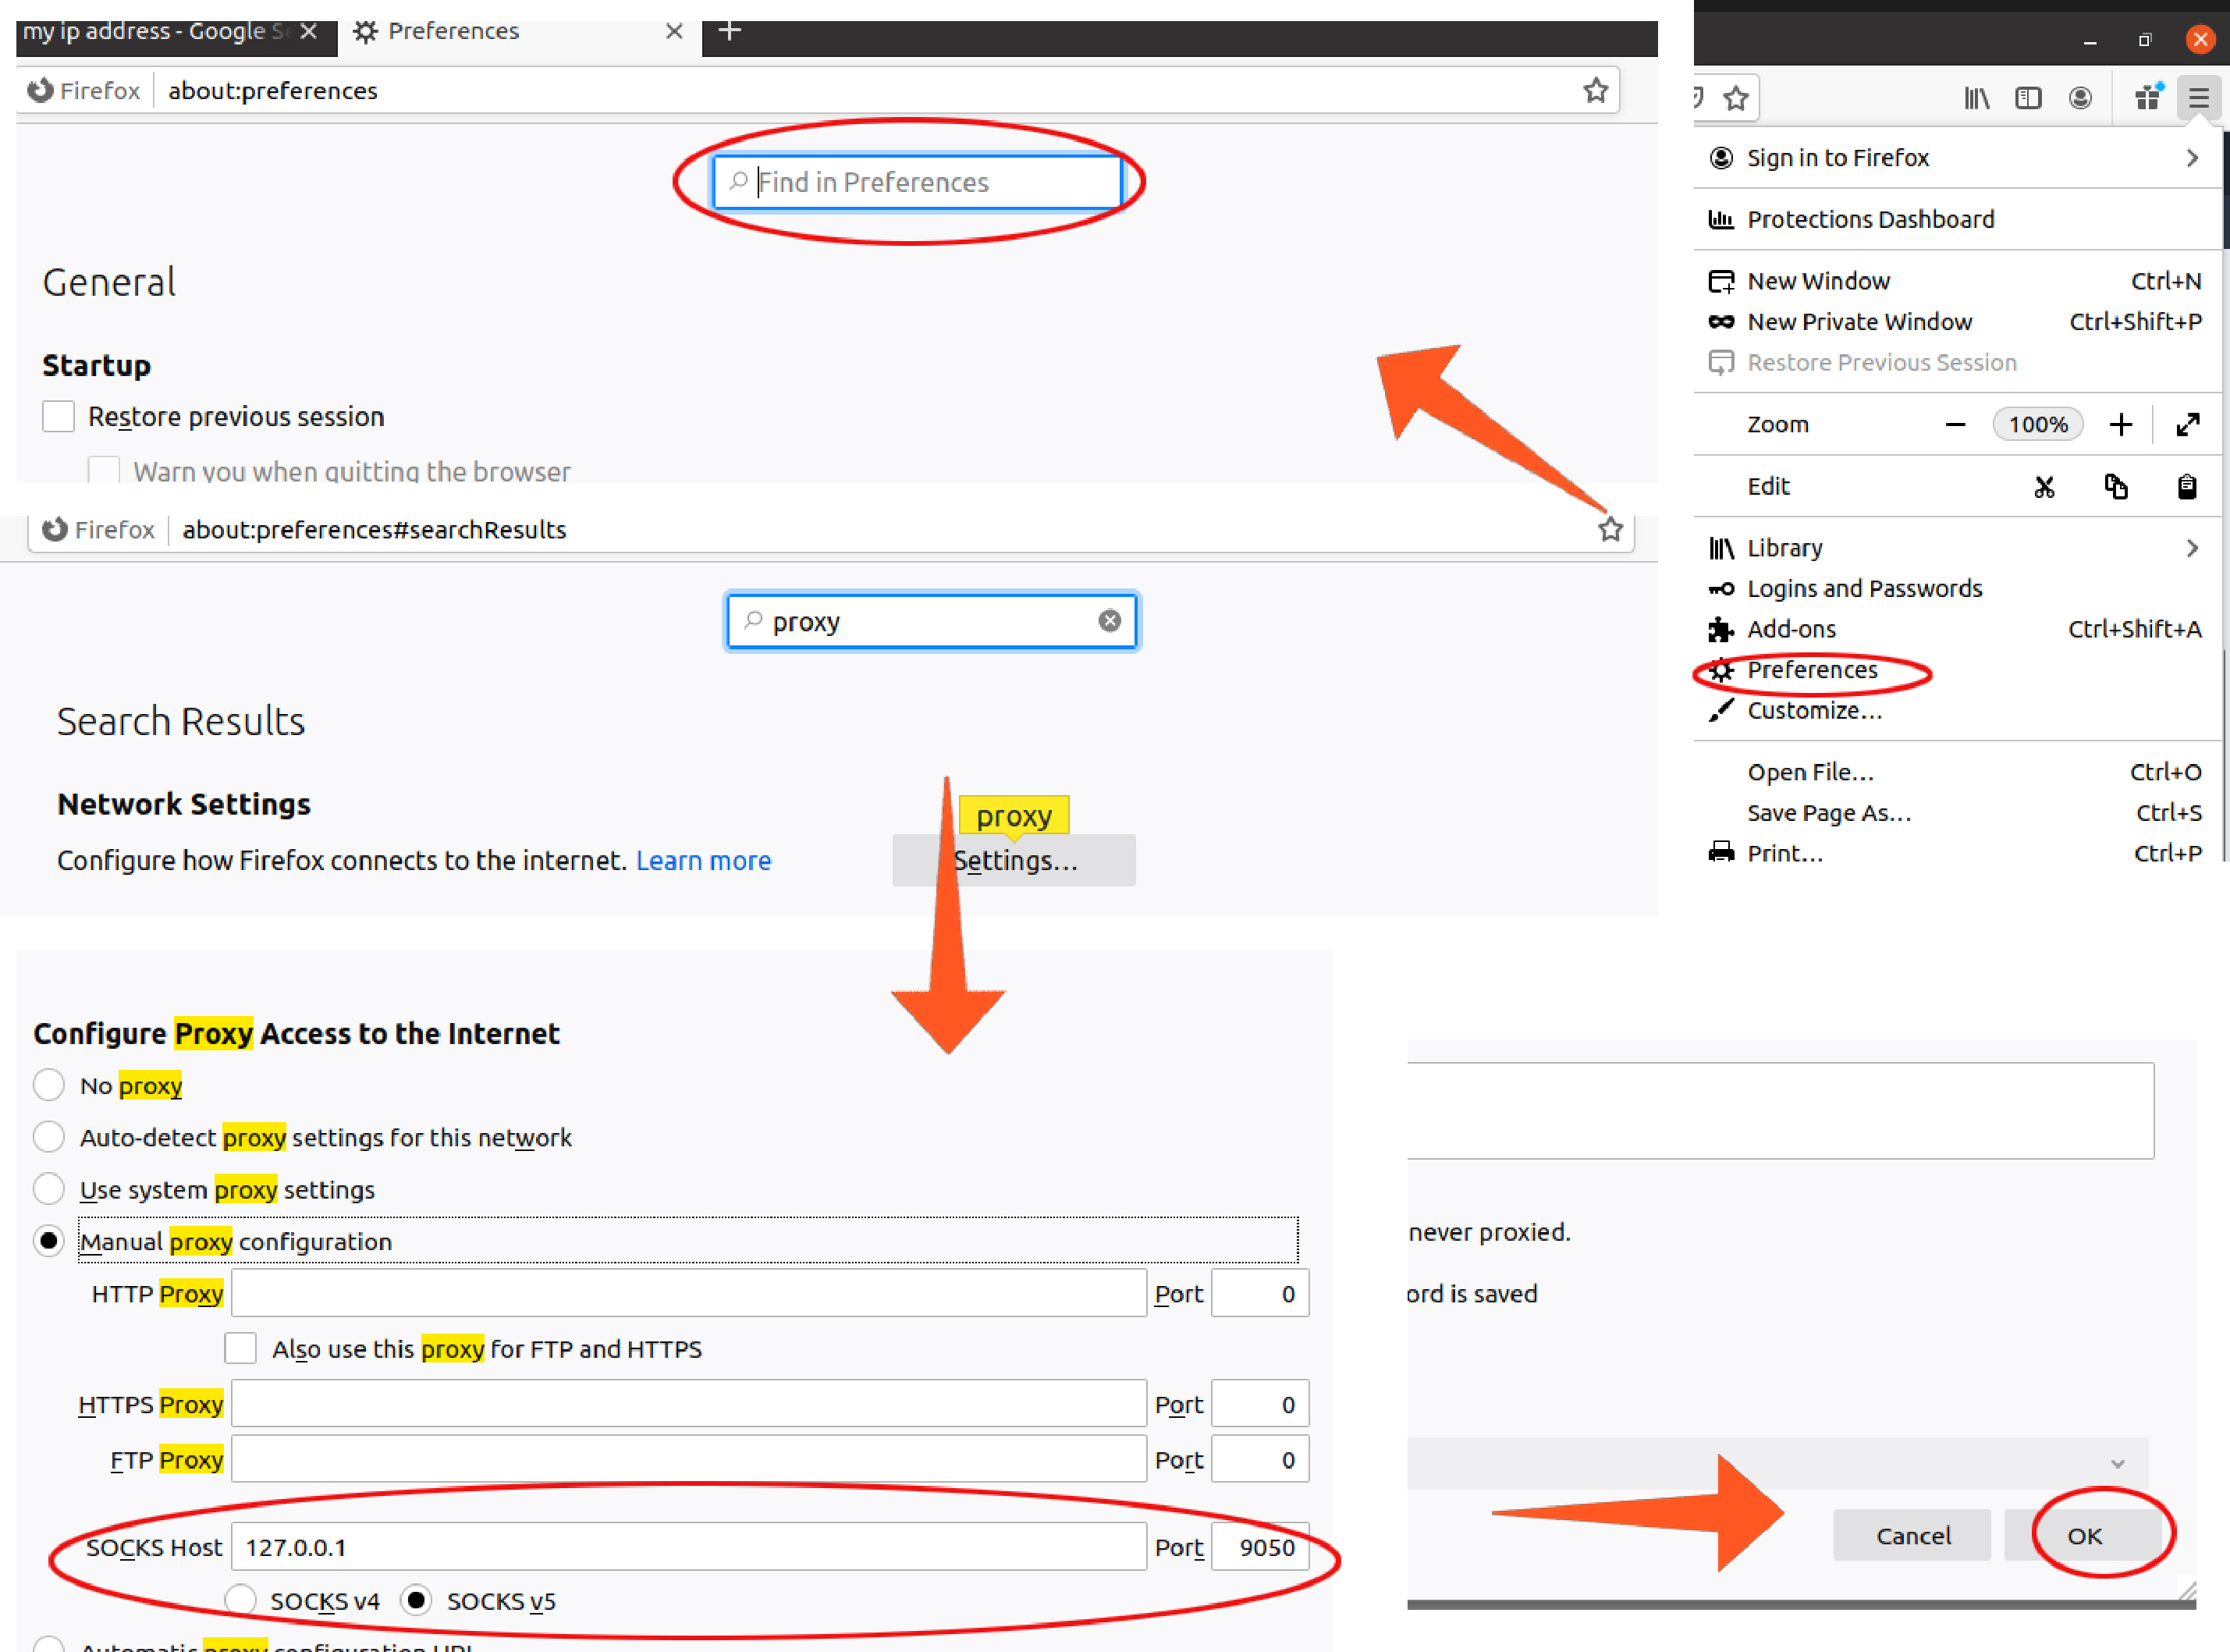
\includegraphics[width=0.8\columnwidth]{proxyenable.pdf}}
\caption{Enabling Proxy}\label{fig:proxyenable}
\end{figure}

\item Use your \textsf{Firefox} to visit \url{https://whatismyipaddress.com/} to check your IP address.  

\textbf{Question 2.} \textbf{Question 2.}  Put a screenshot into your report to show the IP address displayed in your \textsf{Firefox}. Explain what you observed (10 points)..

\item Stop the \tor services using following command and disable Poxy (See \autoref{fig:proxydisable})
 \begin{lstlisting}
$ sudo service tor stop
\end{lstlisting}\vspace{-6mm}

\begin{figure}[h]
\centering
\frame{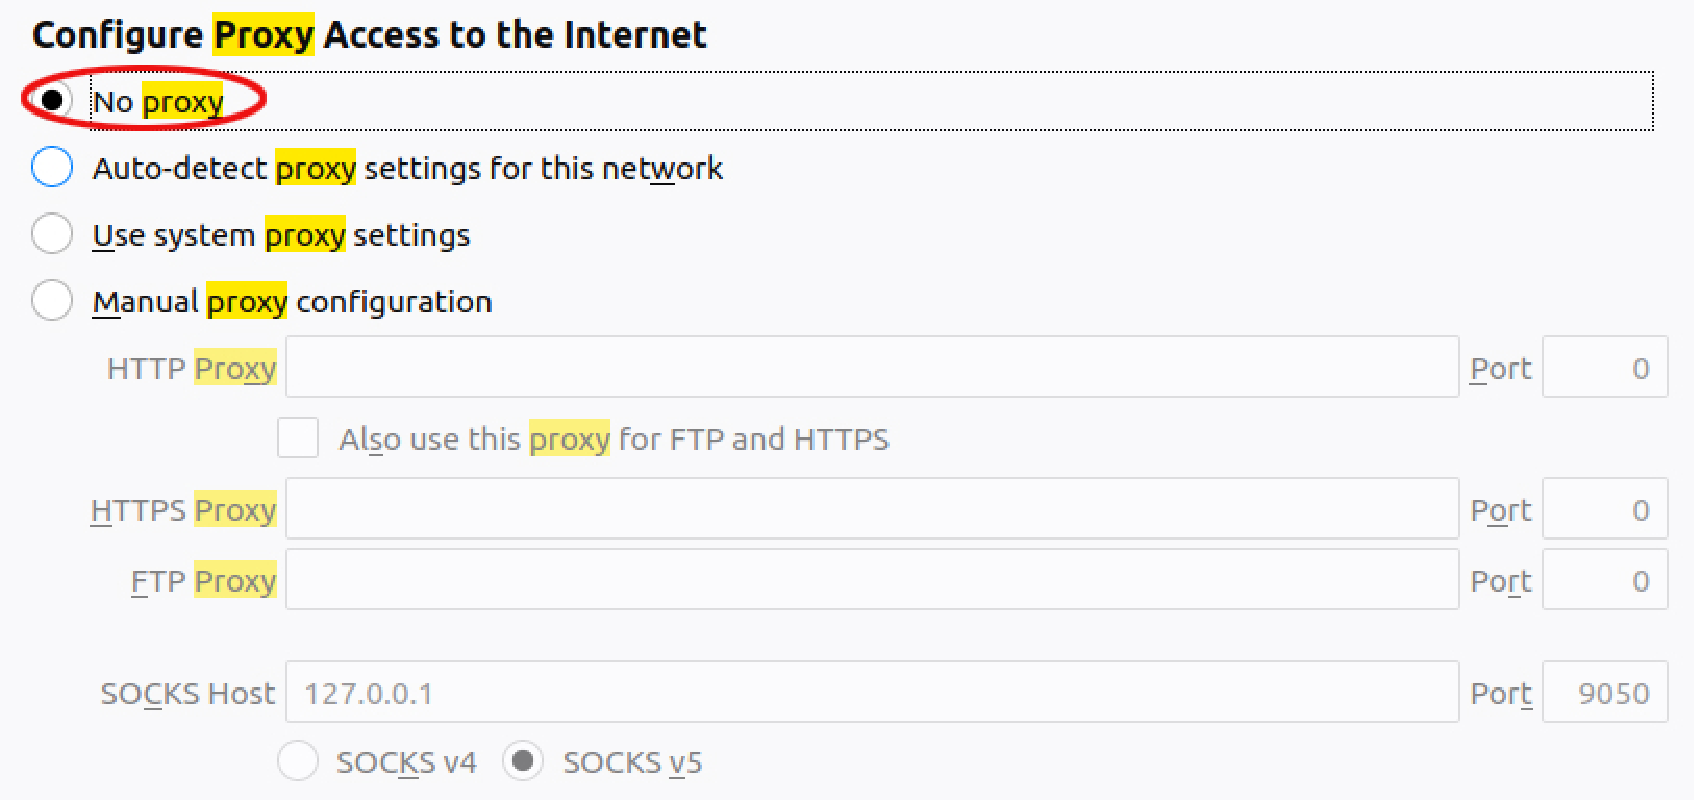
\includegraphics[width=0.8\columnwidth]{proxydisable.pdf}}
\caption{Disabling Proxy}\label{fig:proxydisable}
\end{figure}

\item Use your \textsf{Firefox} to visit \url{https://whatismyipaddress.com/} to check your IP address.

\textbf{Question 3.}  Are the IP addresses displayed in step 5 and step 7 the same? If not, explain why (10 points). 

\end{enumerate}




%\section{Description}
%\begin{enumerate}
%\item \textbf{SQL injection} vulnerabilities are very serious flaws which open applications up to a whole host of database attacks. These vulnerabilities affect more than just web based applications and often allow the circumvention of authentication/access controls for information stored in a database. Also, SQL injection flaws can sometimes be a stepping stone used by attackers to fully compromise a database server. You could find more information about SQL injection in Section~\ref{reference}.

%\item \textbf{Cross-site scripting} vulnerabilities are also quite common in web applications. These flaws allow you to expose the interaction between users and a website. Read more about the different forms of XSS and how they are typically exploited through the provided references in Section~\ref{reference}.

%\item \textbf{Shell command injection}: while somewhat rare, can be devastating to an application's security because these kinds of flaws generally allow remote execution of code and are usually easy to exploit.The problem usually lies in an application's use of external commands to accomplish certain tasks. Often, for the convenience of it, programmers will run external commands via the system shell or some equivalent interface. However, if a user input is included in such commands (for instance, as command line parameters), then it is very difficult to prevent shell meta-character injection. Read more about these attacks and how they can be prevented in Section~\ref{reference}.\end{enumerate} \section{Set up the environmen

\section{Understanding the Security and Privacy in Bluetooth (50 Points)}



%You can use the environment that set up in Lab \#2. If you do not have it, please follow the instruction below to set up one. 
\subsection{Install \textsf{nRF Connect}}
\begin{itemize}
\item  Please open your App Store (or Google Play for Android users) and search a mobile app named \textsf{nRF Connect} (See \autoref{fig:rfconnect}). 
\item Install the app onto your iPhone or Android Phone. \textsf{nRF Connect} is a tool that enables Bluetooth Low energy traffic analysis.  
\end{itemize}

 \begin{figure}[h]
\centering
\frame{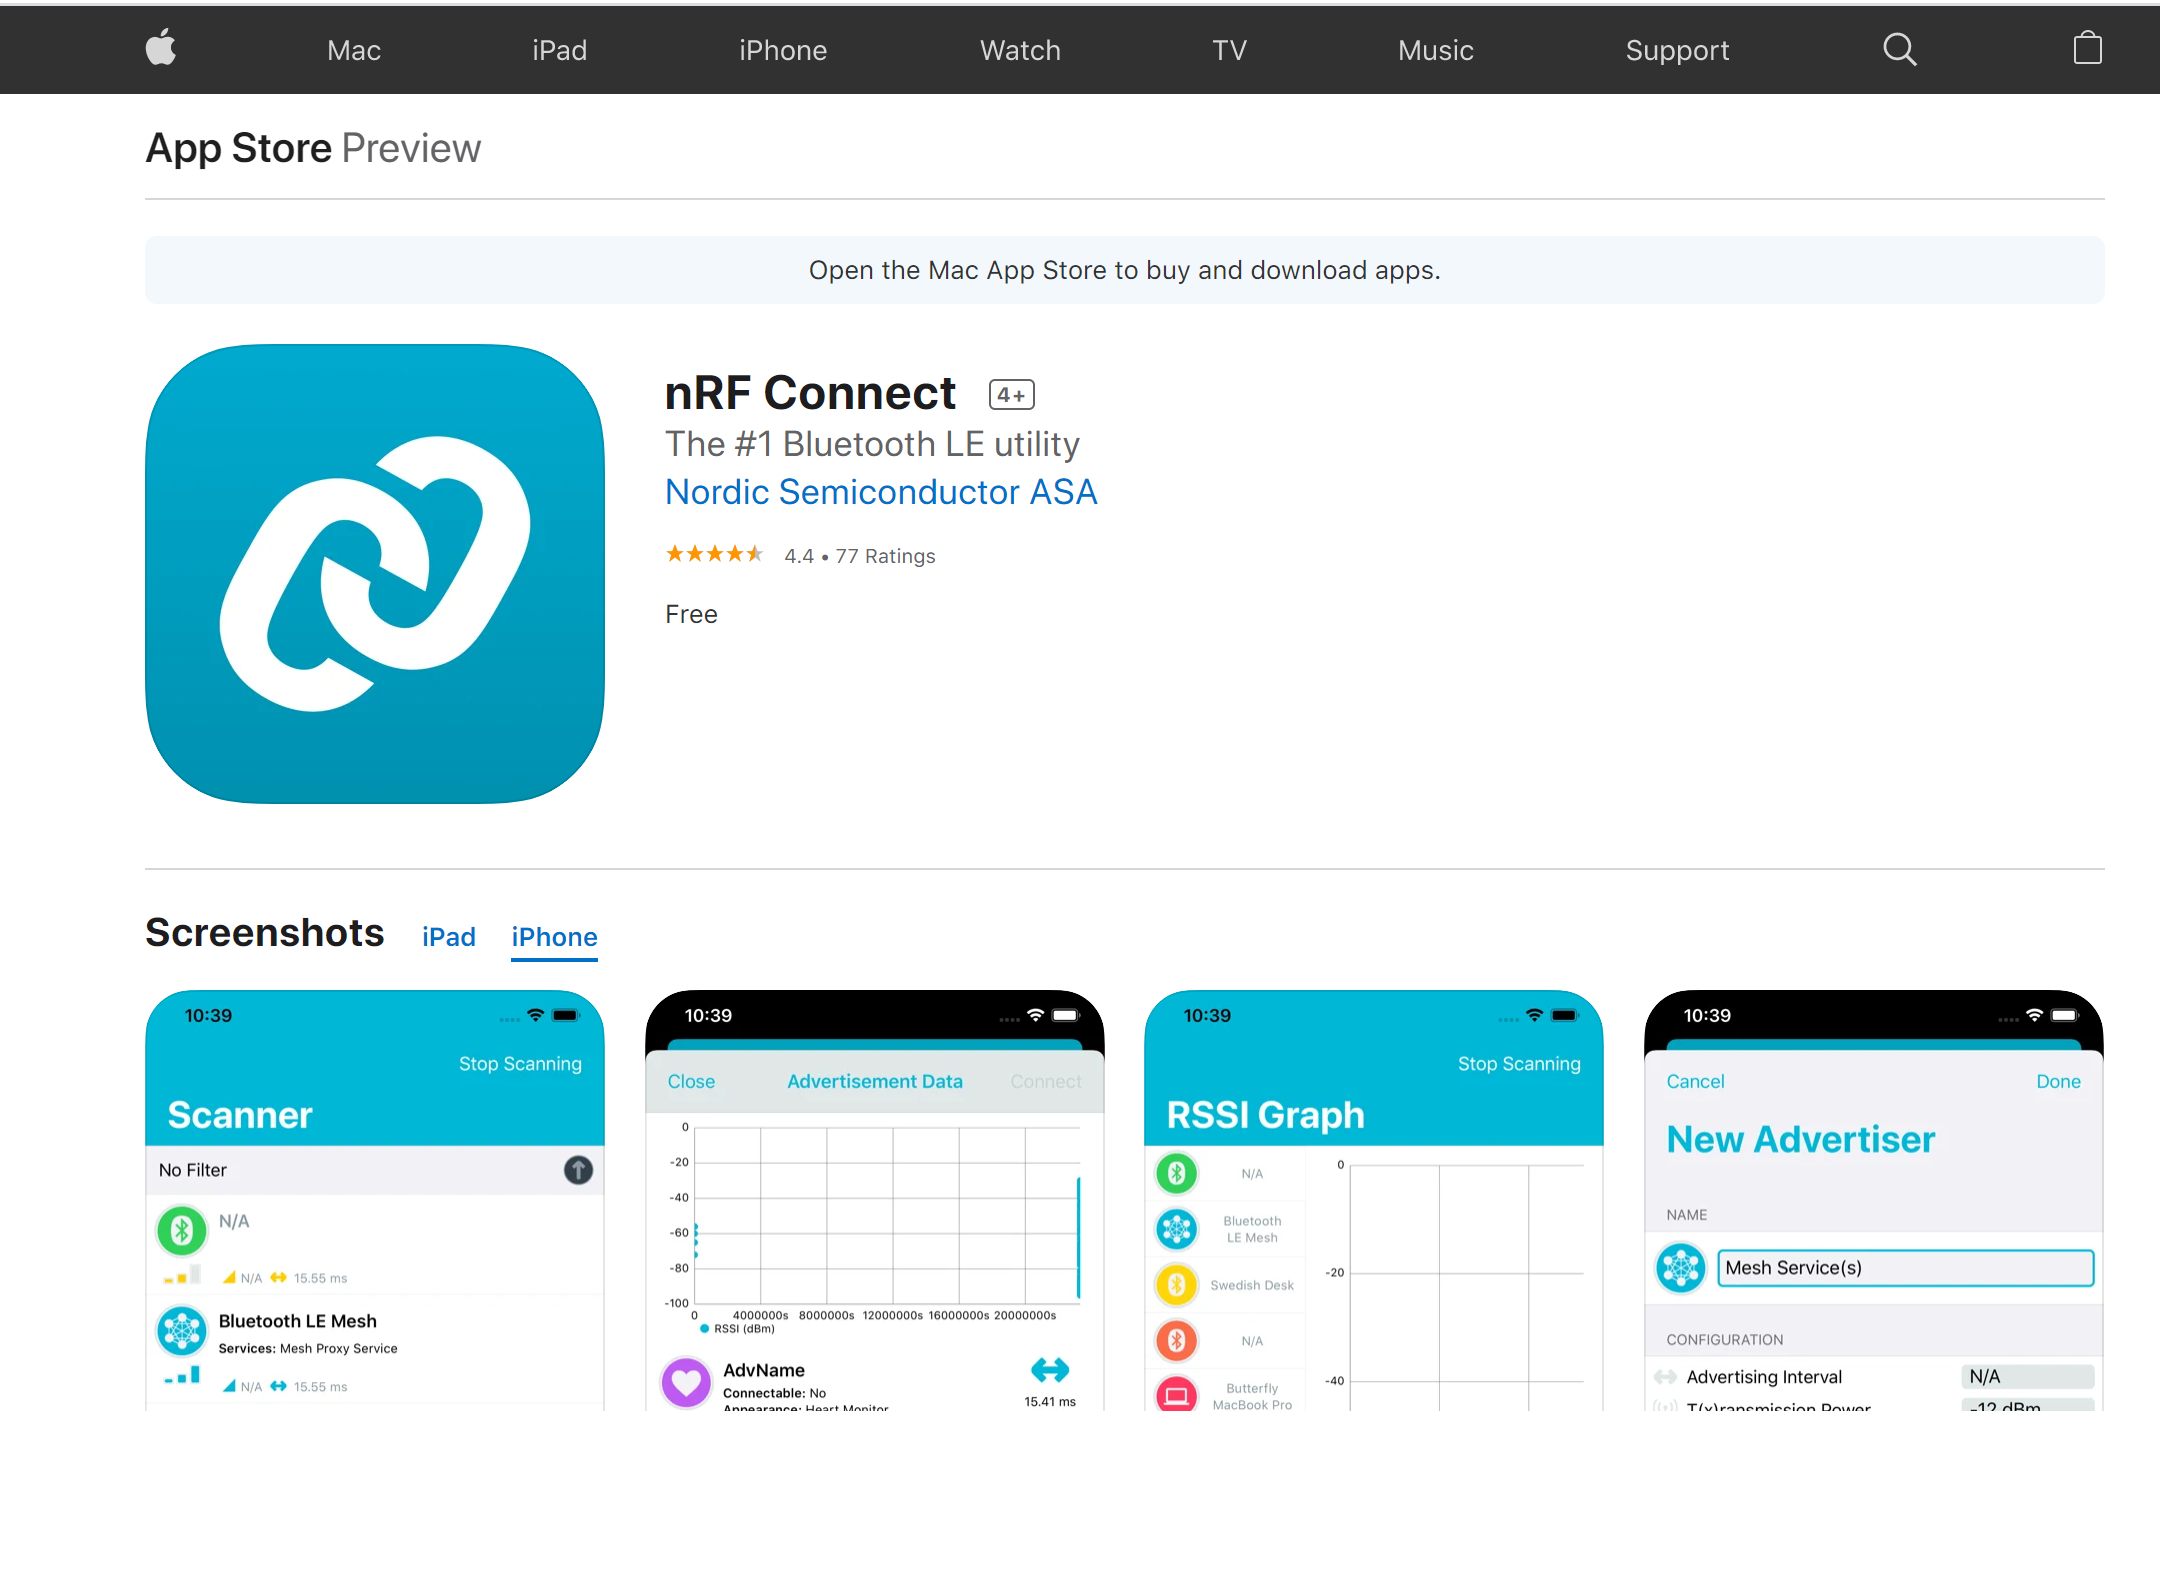
\includegraphics[width=0.7\columnwidth]{rfconnect.png}}
\caption{nRF Connect}\label{fig:rfconnect}
\end{figure}

  
\end{enumerate}





\subsection{Using mobile sniffer to observe the nearby Bluetooth Low Energy (BLE) devices (10 Points)} 
\begin{enumerate}
\item Open \textsf{nRF Connect}. \textsf{nRF Connect} will list the nearby BLE devices. 
\item Check the manufacture data and MAC addresses of nearby BLE devices. The manufacture data will reveal the manufacturers of the BLE devices. Please note that iOS does not support viewing the MAC addresses of other BLE devices. 

 \begin{figure}[h]
\centering
\frame{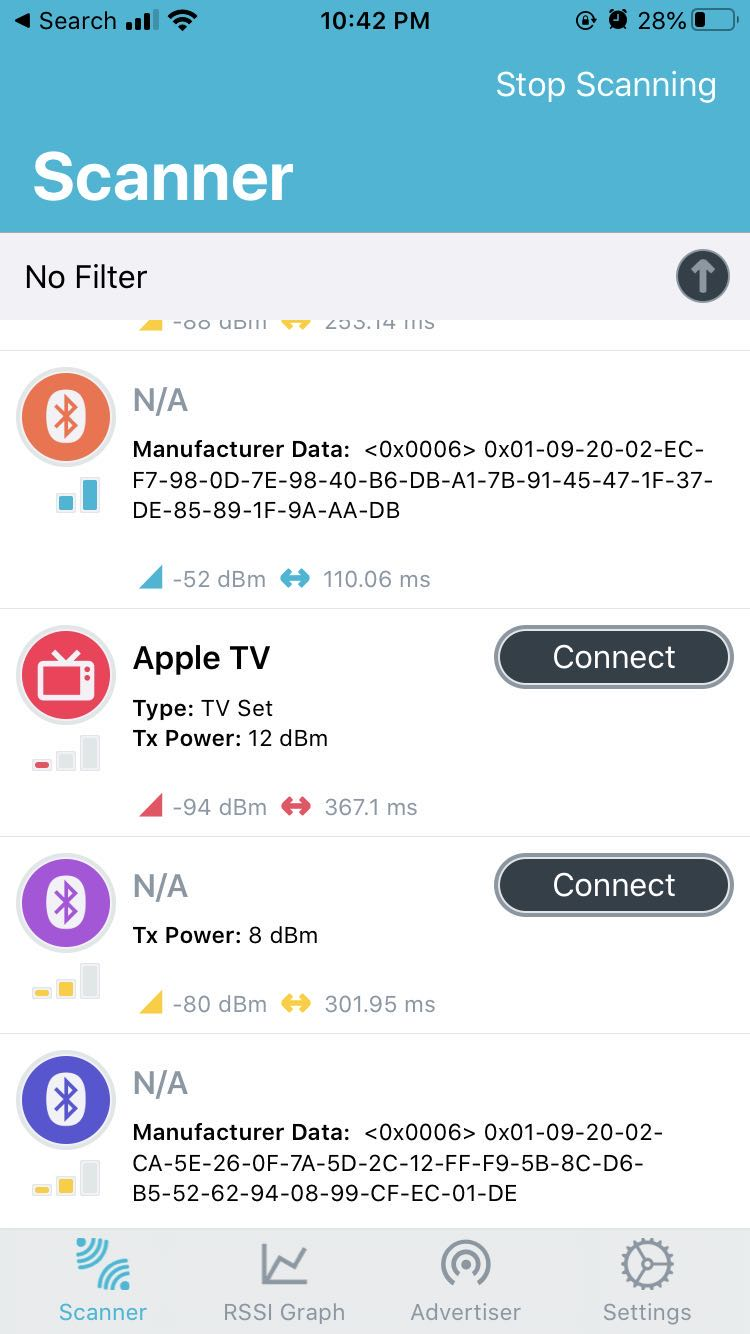
\includegraphics[width=0.4\columnwidth]{scanner.jpg}}
\caption{\textsf{Nearby Bluetooth devices discovered by \textsf{nRF Connect}}}\label{fig:nearbydevice}
\end{figure}
\textbf{Warnings}: Do not attempt to connect other BLE devices, since it may be the violation of ethics.

\textbf{Question 1.} Put a screenshot into your report to show the BLE devices you have observed (10 points). 

\end{enumerate}

\subsection{Analyzing the captured packets (30 Points)}

\begin{enumerate}
\item Please log in your analysis platform using the provided username and password. 
\item Run \textsf{Wireshark}.
 \begin{lstlisting}
$ wireshark
\end{lstlisting}\vspace{-6mm}
\item Configure your \textsf{Wireshark} to view Bluetooth packets. 
\begin{itemize}
\item Edit $\longrightarrow$ Preferences $\longrightarrow$ Protocol $\longrightarrow$ DLT\_USER (See \autoref{fig:wiresharkconfig}) 
\item Configure the encapsulation Table. Particularly, ``DLT'' should set to ``147'' and the payload protocol should set to ``btle''. 
\end{itemize}

\begin{figure}[h]
\centering
\frame{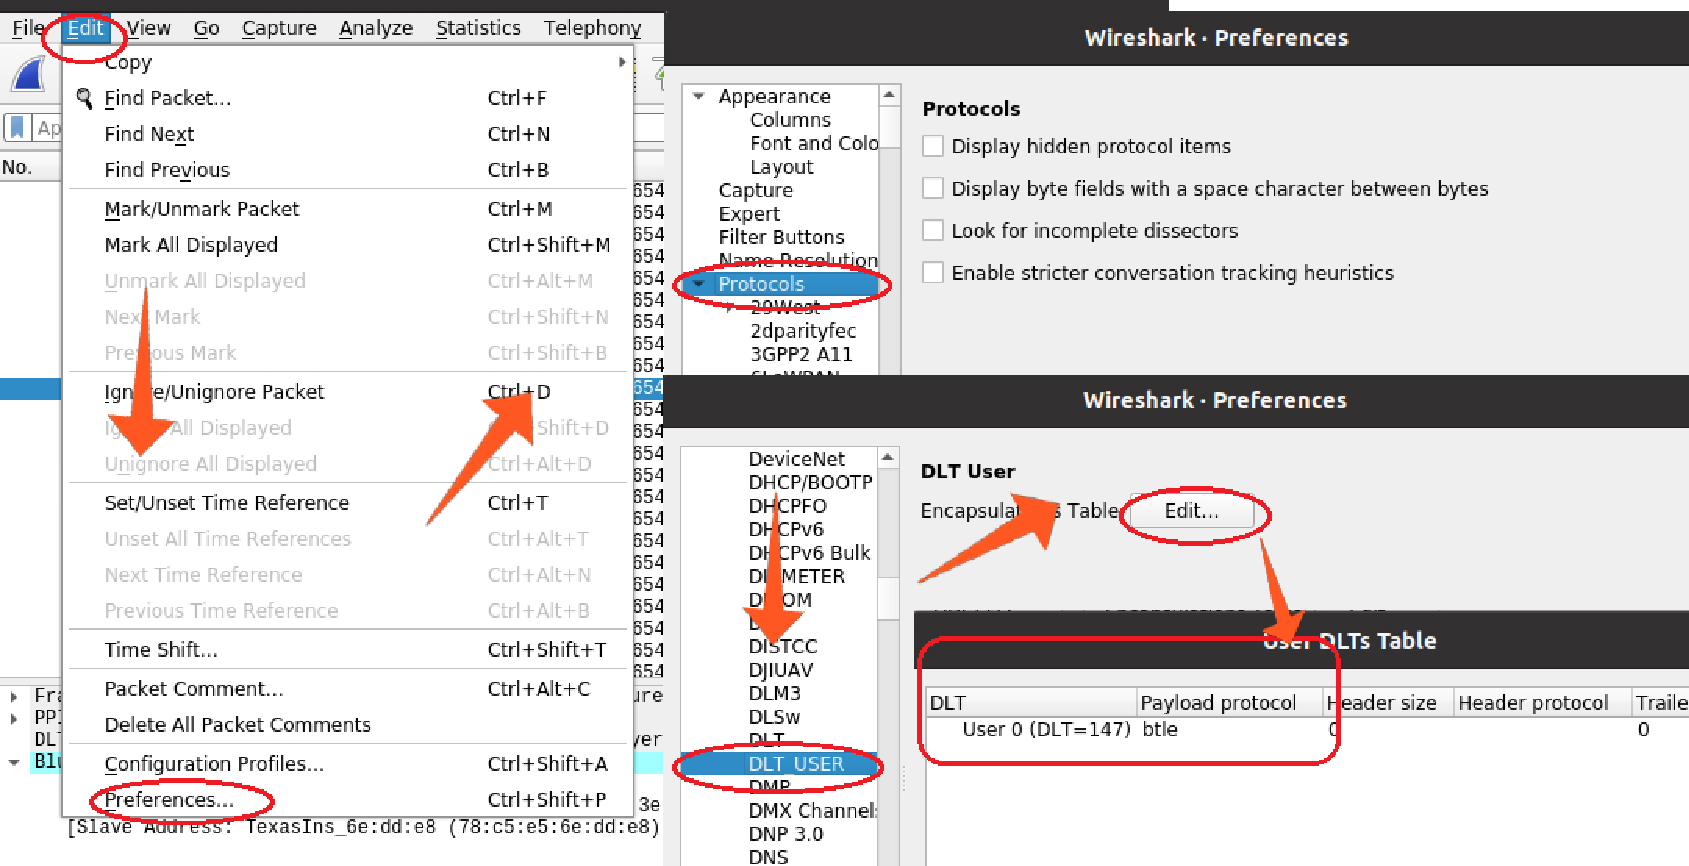
\includegraphics[width=0.8\columnwidth]{wiresharkconfig.pdf}}
\caption{\textsf{Configure \textsf{Wireshark}}}\label{fig:wiresharkconfig}
\end{figure}


\item Download the ``blepcap.pcap'' file at \url{https://drive.google.com/file/d/18iQ2MfIQYmQs8WOcRztuHce1W6YQSubp/view?usp=sharing}. Use \textsf{wireshark} to view the content. 

\item Identify the types of the Bluetooth packets. In the example, there are 5 types of Bluetooth packets, including advertising packets (i.e., \textsf{ADV\_IND}), scan request packets (i.e., \textsf{SCAN\_REQ}), scan response (i.e., \textsf{SCAN\_RSP}), connection request (i.e., \textsf{CONNECT\_REQ}) packets, and data exchanging packets.


\textbf{Question 1.} Check the format of advertising packets (i.e., \textsf{ADV\_IND}) and answer the following question (10 Points):
\begin{itemize}
\item What is the MAC address of the broadcasting device (3 points)? 
\item What is the manufacture data of the broadcasting device (3 points)?
\item What is the UUID of the broadcasting devices (4 points)?
\end{itemize}

\textbf{Question 2.} Check the format of scan request packets (i.e.,  \textsf{SCAN\_REQ}) and answer the following question (10 Points):
\begin{itemize}
\item What is the MAC address of the initiating device in \textsf{SCAN\_REQ} (5 points)?
\item What is the MAC address of the device that the initiating device attempts to scan in \textsf{SCAN\_REQ}  (5 points)?
 
\end{itemize}

 

\textbf{Question 3.}  What are the security requirements of the broadcasting device (10 Points)? 

\textbf{Tip:} Security requirements of a device can be observed in pairing response packets, which is a special type of data exchanging packet  (See \autoref{fig:requirement}). 
 
\begin{figure}[h]
\centering
\frame{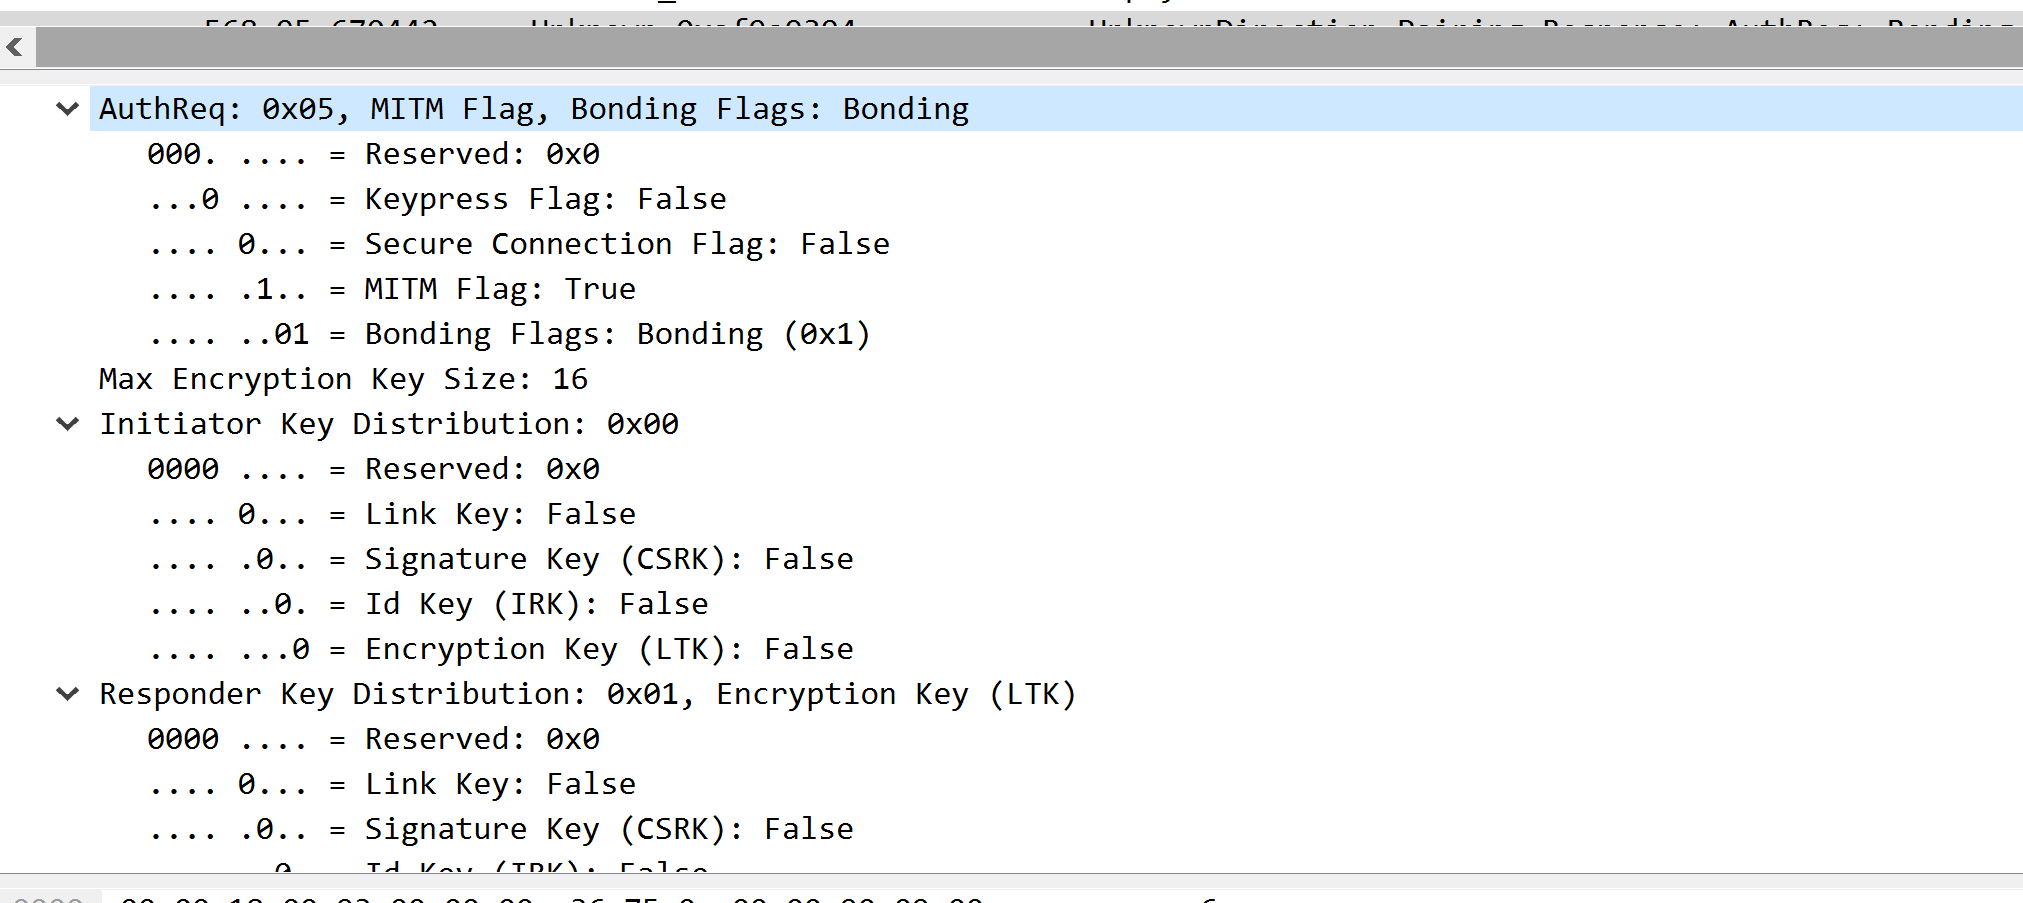
\includegraphics[width=0.8\columnwidth]{mitmcheck.png}}
\caption{\textsf{Checking security requirements of a device}}\label{fig:requirement}
\end{figure}  

\end{enumerate}


\subsection{Install \textsf{Crackle} and Decrypt encrypted Bluetooth packets (10 Points)}


\begin{enumerate}
 
\item Go to the directory of \textsf{Crackle} and type: 
 \begin{lstlisting}
$ make 
$ make install
\end{lstlisting}\vspace{-6mm}

\item Download and unzip the testing samples at \url{http://lacklustre.net/bluetooth/crackle-sample.tgz}.
\item Identify \textsf{Just Works} Pairing:
 \begin{lstlisting}
$ crackle -i ltk_exchange.pcap
\end{lstlisting}\vspace{-6mm}

\textbf{Question 1.} Put a screenshot into your report to show you have identified  \textsf{Just Works} Pairing (5 points). 

\item View encrypted Bluetooth packets in file \texttt{encrypted\_known\_ltk.pcap} using \textsf{Wireshark}. It can be observed that once connected, the data exchanging packets are unreadable (See \autoref{fig:envsde}). 
 
 
\item Decrypt the Bluetooth packets using a given long term key (LTK):
 \begin{lstlisting}
$ crackle -i encrypted_known_ltk.pcap -o decrypt.pcap -l 7f62c053f104a5bbe68b1d896a2ed49c
\end{lstlisting}\vspace{-6mm}

\item View the decrypted Bluetooth packets in file \texttt{decrypt.pcap} using \textsf{Wireshark}. We can see the GATT read request now. 

\begin{figure}[h]
\centering
\frame{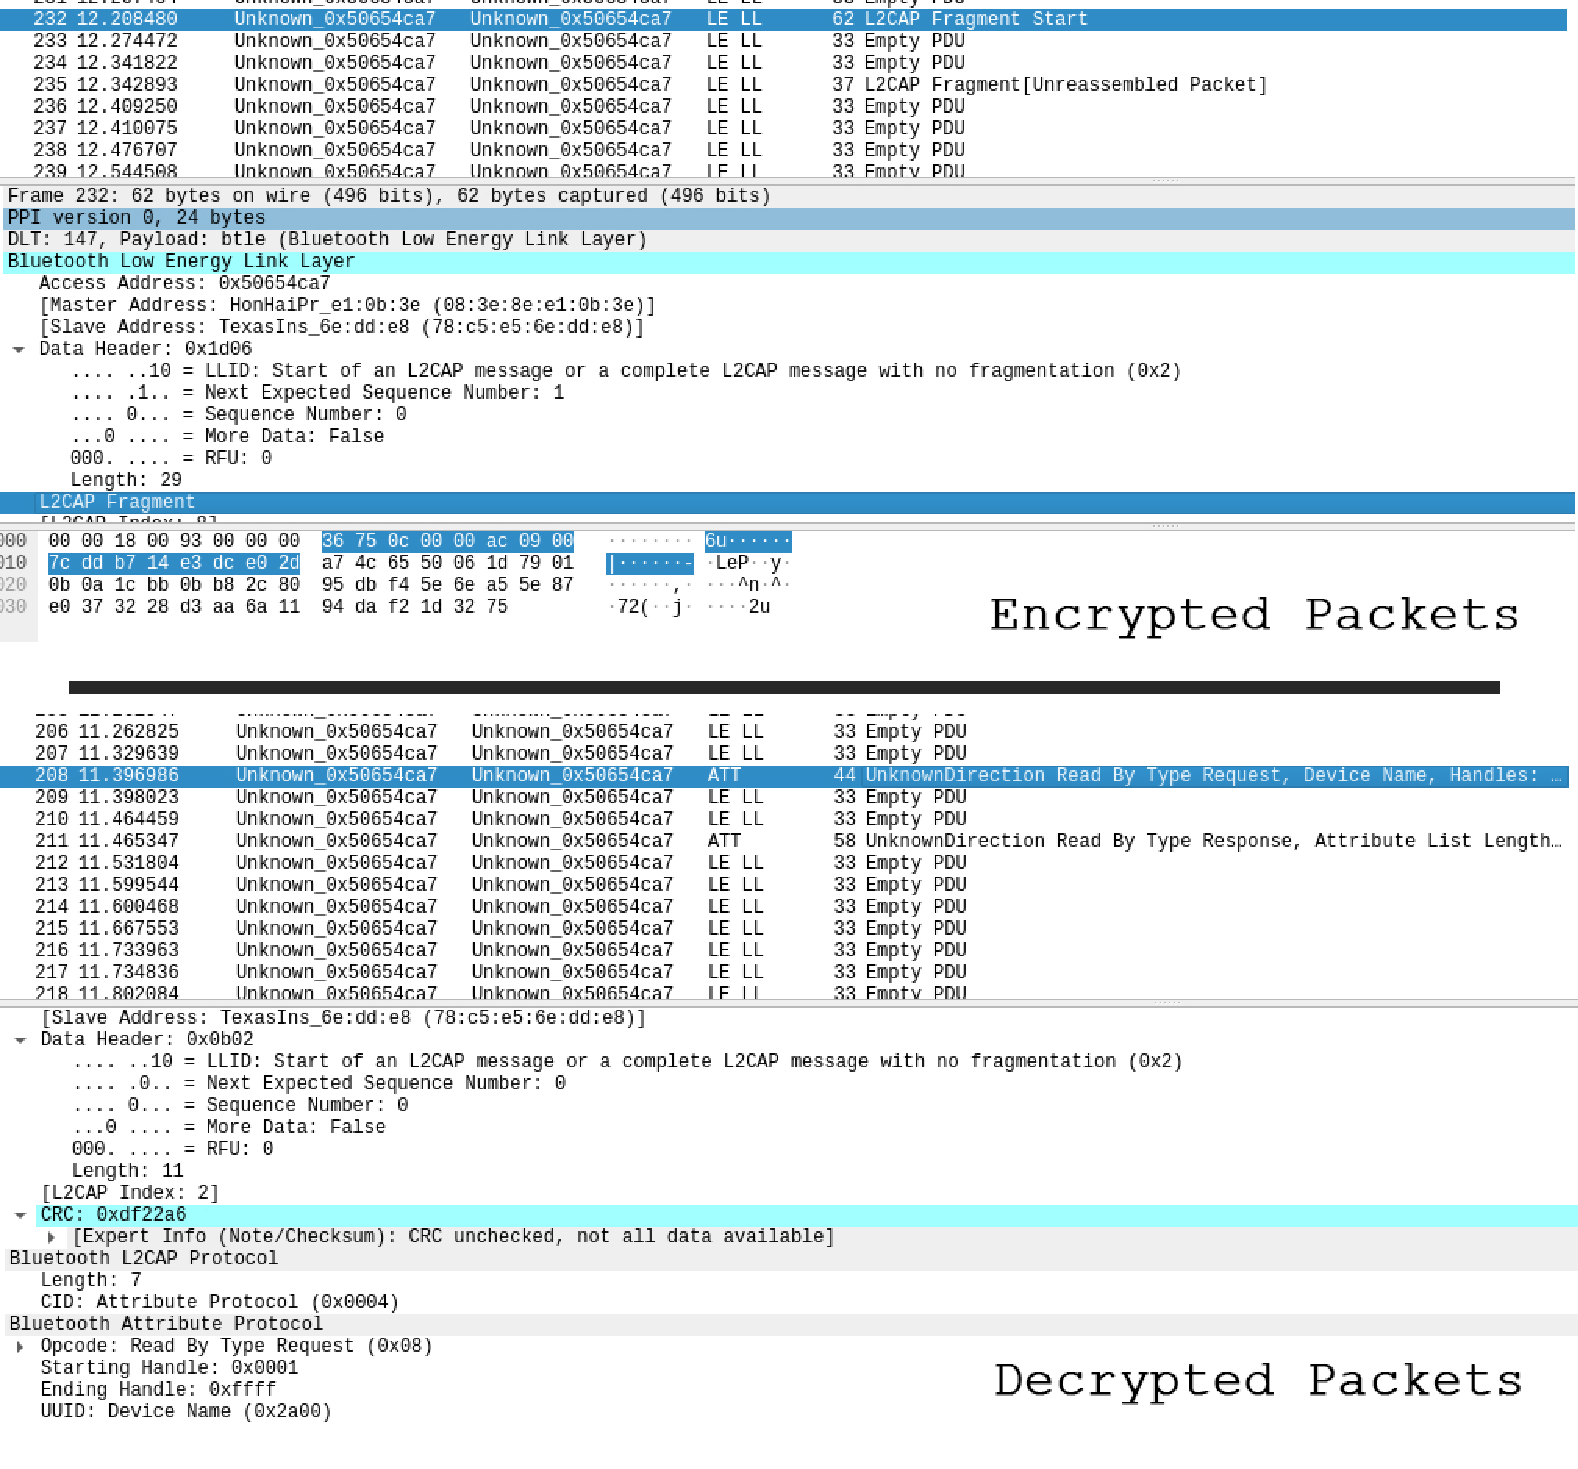
\includegraphics[width=0.8\columnwidth]{envsde.pdf}}
\caption{\textsf{Encrypted packets v.s. decrypted packets}}\label{fig:envsde}
\end{figure}

 

\textbf{Question 1.} Put screenshots into your report to show you have decrypt the Bluetooth packets successfully (5 points). 
\end{enumerate}  


\section{Submit Your Lab Report}
\label{deliver}
Please write a report describing how you solve each of the problem above, and submit at CARMEN.

\section{Code of Conduct}

These labs are intended for educational purposes only, to provide a safe and legal means to gain an understanding of security by understanding threats and vulnerabilities. They are not intended for (and are not to be used for) any purposes other than for education. 

Some of these labs are based on existing exploits, and students are to exploit their own virtual machines ONLY. Do not try them outside your personal devices. Use of anything learned in, during, or resulting from this class that is in any manner illegal, unauthorized, or unethical is forbidden. There are serious consequences for illegal computer hacking. Any student who violates the rules is subject to legal action, will take sole responsibility of his/her actions, and cannot hold any claim on the responsibility of the faculty, staff, or the university. Students who violate these conditions of the labs will get a failing grade in the class and may be subject to legal action. 
Do not incorporate or implement viruses, worms, spyware and/or Trojan horses in ANY of these labs. Only the tools and resources specified in the given lab may be used. Any student who exploits fellow student's accounts or gains the solutions to the labs by means other than specified is engaging in academic misconduct. Academic misconduct will be treated seriously. 
  

\end{document}

